We train SOMs using four different topologies:
\emph{rectangular, hexagonal, geodesic sphere} and \emph{spherical}.  The spherical
topology is based on a method, developed by \cite{Rakhmanov94}, for
distributing an arbitrary number of points on to the surface of a sphere.
Delaunay triangulation is then applied to these points, producing a
topological structure.  To yield meaningful results these SOMs must be trained
with comparable parameters.  The literature provides many rules of thumb for
training a SOM: each SOM is trained in two stages, the first of which uses a larger
initial learning rate and neighborhood search radius with a small number of
training steps; the second stage uses a lower initial learning rate and
neighborhood search radius, but extends the length of training.
\\
First Stage Parameters:
\begin{itemize}
  \item Initial neighborhood search radius of 50\%, which decreases during training. 
  \item Initial learning rate of 0.04 which decreases during training.
  \item 100,000 training steps.
\end{itemize}
Second Stage Parameters:
\begin{itemize}
  \item Initial neighborhood search radius of 33\%, which decreases during training. 
  \item Initial learning rate of 0.03 which decreases during training.
  \item 1,000,000 training steps.
\end{itemize}

As shown in Figure \ref{fig:nSize}, topologies differ in terms of achievable
network size.  For comparability, the network size of each SOM needs to be as
close as possible.  The achievable network size for the geodesic SOM is the
most limiting of the topologies we test. We chose the eighth frequency
geodesic sphere, which has 642 nodes, which is relatively close to the
644-node hexagonal and rectangular topologies achieved when the dimensions are
set to \(28x23\). Finally, the spherical topology was set to 642 nodes.

\begin{figure}[htb]
  \begin{center}
\caption{SOM Size and spherical topologies.}
\label{fig:nSize}
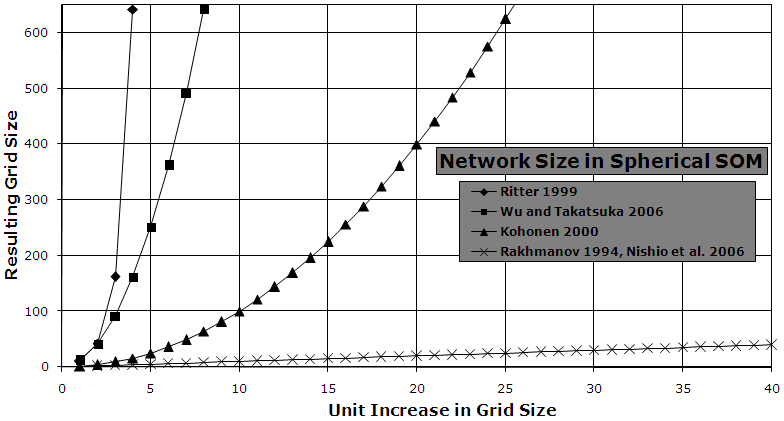
\includegraphics[width=0.70\linewidth]{networkSize.png}
\end{center}
\end{figure}


